\section{Expressions}
\label{sec:Expressions}
This part of the language describes expressions. Expressions are in The Language Described in This Report defined as the constructs that have a value. These can be used together with specific operators to create larger expressions as one would do in mathematics. Apart from combining expressions they are often used as the right hand side of an assignment, but can also be used for indexing, the condition in conditional statements, for return values and in general all places where a value is expected.

\subsection{Operators}\label{subsec:operators}
First we look at the mathematical operators that can combine expressions.
\setlength{\grammarindent}{100pt}
\begin{grammar}
<Expression> ::= <Expression> <PSEVENOPERATOR> <OP7>
 \alt <OP7>

<OP7> ::= <OP7> <PSIXOPERATOR> <OP6>
 \alt <OP6>

<OP6> ::= <OP6> <PFIVEOPERATOR> <OP5>
 \alt <OP5>

<OP5> ::= <PFOUROPERATOR> <OP5>
 \alt <OP4>

<OP4> ::= <OP4> <PTHREEOPERATOR> <OP3>
 \alt <OP3>

<OP3> ::= <OP3> <PTWOOPERATOR> <OP2>
 \alt <OP2>

<OP2> ::= <OP2> <PONEOPERATOR> <OP1>
 \alt <OP1>

<OP1> ::= <PZEROOPERATOR> <OP1>
 \alt <OP0>

<OP0> ::= <Operand>
 \alt '(' <Operation> ')'

<PZEROOPERATOR> ::= '(''int' | 'real' | 'char' | 'bool'')'

<PONEOPERATOR> ::= '$\Twedge$' | '\#'

<PTWOOPERATOR> ::= '*' | '/' | '\%'

<PTHREEOPERATOR> ::= '+' | '-'

<PFOUROPERATOR> ::= '=' | '!=' | '$\textless$' | '$\textless$=' | '$\textgreater$' | '$\textgreater$='

<PFIVEOPERATOR> ::= 'NOT'

<PSIXOPERATOR> ::= 'AND' | 'NAND'

<PSIXOPERATOR> ::= 'OR' | 'XOR' | 'NOR'
\end{grammar}
The precedence of the operators are created in the grammar. Here the parse tree will be created, such that the $\braket{PSEVENOPERATOR}$ is placed highest in the tree and the $\braket{PZEROOPERATOR}$ is placed lowest as standard, meaning that the precedence goes from $\braket{PZEROOPERATOR}$ to $\braket{PSEVENOPERATOR}$ with zero having highest precedence. This precedence can be overwritten by parentheses that resets the order so expressions inside parentheses are placed lowest in the tree. All operators have left associativity. An example can be seen in \cref{precedenceExamples} this shows how the parse tree is created from the expression: \\
\begin{center}
$\Tnot a \Tand b \Txor 2 < 3 * (2 + 2) + 4$
\end{center}

\begin{figure}[h]
\centering
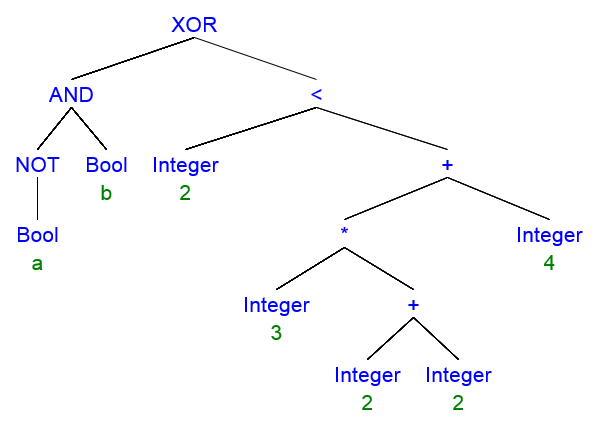
\includegraphics[width=0.7\textwidth]{Design/Expressions/precidenceExamples.png}
\caption{The parse tree for \textnormal{\enquote{$\Tnot a \Tand b \Txor 2 < 3 * (2 + 2) + 4$}}} %[XOR [AND [NOT [Bool a]][Bool b]] [< [Integer 2] [+ [* [Integer 3] [+ [Integer 2] [Integer 2]]] [Integer 4]]]]
\label{precedenceExamples}
\end{figure}

We can see that the operator placed lowest in the tree is \enquote{+} even though \enquote{*} has a higher precedence, and should there for be lower in the tree. This is done because the parentheses overwrites the the order so that everything inside gets higher precedence as intended. If we insert parentheses to illustrate the implicit precedence in the expression it would look like this:
\begin{center}
$((\Tnot a) \Tand b) \Txor (2 < ((3 * (2 + 2)) + 4))$
\end{center}
In \cref{precedenceExamples} we can see that the \enquote{XOR} operator is placed highest in the tree meaning that it has the lowest precedence. We can also see from the tree that this operator takes the result from \enquote{AND} and \enquote{<} as arguments where \enquote{<} again takes the result from \enquote{+} and the integer 2 as arguments and so on. We can see that the arguments changes type as we traverse the tree. We now look at the semantics and what impact this has on the formal type rules.

\subsubsection{Arithmetic Expressions}

First we look at arithmetic expressions. Arithmetic expressions are in TLDR defined as expressions that evaluates to a number, either a real or integer. The operators that creates the arithmetic expressions are +, -, *, /, \%, $\Tpot$ and \#. The semantics for these operators are as follows:

\begin{itemize}
\item "+" is a binary operator that adds two numbers of the same type

\begin{align*}
&\inference[$\text{ADD}_\text{L}$]{e \vdash a_1 \Rightarrow_A a_1'}
                    {e \vdash  a_1 + a_2 \Rightarrow_A a_1' + a_2}
&
&\inference[$\text{ADD}_\text{R}$]{e \vdash a_1 \Rightarrow_A a_1'}
                    {e \vdash a_2 + a_1 \Rightarrow_A a_2 + a_1'}
\\\\
&\inference[$\text{ADD}_\text{V}$]{}
                    {v_1 + v_2 \Rightarrow_A v}
                    {, v_1 + v_2 = v}
\end{align*}

\item "-" is a binary operator that subtracts two numbers of the same type

\begin{align*}
&\inference[$\text{SUB}_\text{L}$]{e \vdash a_1 \Rightarrow_A a_1'}
                    {e \vdash a_1 - a_2 \Rightarrow_A a_1' - a_2}
&
&\inference[$\text{SUB}_\text{R}$]{e \vdash a_1 \Rightarrow_A a_1'}
                    {e \vdash a_2 - a_1 \Rightarrow_A a_2 - a_1'}
\\\\
&\inference[$\text{SUB}_\text{V}$]{}
                    {v_1 - v_2 \Rightarrow_A v}
                    {, v_1 - v_2 = v}
\end{align*}

\item "*" is a binary operator that multiplies two numbers of the same type

\begin{align*}
&\inference[$\text{MULT}_\text{L}$]{e \vdash a_1 \Rightarrow_A a_1'}
                     {e \vdash a_1 * a_2 \Rightarrow_A a_1' * a_2}
&
&\inference[$\text{MULT}_\text{R}$]{e \vdash a_1 \Rightarrow_A a_1'}
                     {e \vdash a_2 * a_1 \Rightarrow_A a_2 * a_1'}
\\\\
&\inference[$\text{MULT}_\text{V}$]{}
                     {v_1 * v_2 \Rightarrow_A v}
                     {, v_1 * v_2 = v}
\end{align*}

\item "/" is a binary operator that divides two numbers of the same type

\begin{align*}
&\inference[$\text{DIV}_\text{L}$]{e \vdash a_1 \Rightarrow_A a_1'}
                    {e \vdash a_1 / a_2 \Rightarrow_A a_1' / a_2}
&
&\inference[$\text{DIV}_\text{R}$]{e \vdash a_1 \Rightarrow_A a_1'}
                    {e \vdash a_2 / a_1 \Rightarrow_A a_2 / a_1'}
\\\\
&\inference[$\text{DIV}_\text{V}$]{}
                    {v_1 / v_2 \Rightarrow_A v}
                    {, \frac{v_1}{v_2} = v}
\end{align*}

\item "\%" is a binary operator that returns the remainder of a floored division of two numbers of the same type

\begin{align*}
&\inference[$\text{MOD}_\text{L}$]{e \vdash a_1 \Rightarrow_A a_1'}
                    {e \vdash a_1 \% a_2 \Rightarrow_A a_1' \% a_2}
&
&\inference[$\text{MOD}_\text{R}$]{e \vdash a_1 \Rightarrow_A a_1'}
                    {e \vdash a_2 \% a_1 \Rightarrow_A a_2 \% a_1'}
\\\\
&\inference[$\text{MOD}_\text{V}$]{}
                    {v_1 \% v_2 \Rightarrow_A v}
                    {, v_1 \;\; \textrm{mod} \;\; v_2 = v}
\end{align*}

\item "\^{}" is a binary operator that lifts the first number to the power of the second number

\begin{align*}
&\inference[$\text{POW}_\text{L}$]{e \vdash a_1  \Rightarrow_A a_1'}
                    {e \vdash a_1 \Twedge a_2 \Rightarrow_A a_1' \Twedge a_2}
&
&\inference[$\text{POW}_\text{R}$]{e \vdash a_1 \Rightarrow_A a_1'}
                    {e \vdash a_2 \Twedge a_1 \Rightarrow_A a_2 \Twedge a_1'}
\\\\
&\inference[$\text{POW}_\text{V}$]{}
                    {v_1 \Twedge v_2 \Rightarrow_A v}
                    {, v_1 ^ {v_2} = v}
\end{align*}

\item "\#" is a binary operator that roots the first operand to the second operand
\begin{align*}
&\inference[$\text{ROOT}_\text{L}$]{e \vdash a_1 \Rightarrow_A a_1'}
                    {e \vdash a_1 \# a_2 \Rightarrow_A a_1' \# a_2}
&
&\inference[$\text{ROOT}_\text{R}$]{e \vdash a_1 \Rightarrow_A a_1'}
                    {e \vdash a_2 \# a_1 \Rightarrow_A a_2 \# a_1'}
\\\\
&\inference[$\text{ROOT}_\text{V}$]{}
                    {v_1 \# v_2 \Rightarrow_A v}
                    {, \sqrt[v_1]{v_2} = v}
\end{align*}

\item "( )" Parenteses gives what they surrounds the highest precedence.

\begin{align*}
&\inference[$\text{PARENS}_\text{A}$]{e \vdash a_1 \Rightarrow_A a_1'}
                       {e \vdash (a_1) \Rightarrow_A (a_1')}
&
&\inference[$\text{PARENS}_\text{V}$]{}
                       {(v) \Rightarrow_A v}
\end{align*}
\end{itemize}

For simplicity we create the following set since all type rules for these are the same.

\begin{center}
$\Taop = \left\{ {+, -, *, /, \%, \; \Tpot \;} \right\}$
\end{center}

Due to the semantics of all \enquote{AOP} operators these can not evaluate to a real if the two inputs are both integers. Therefore all operators in this set can take either two integers and evaluate to an integer or two reals and evaluate to a real.

The \enquote{\#} operator is a bit different. When taking the an integer root of another integer it can still evaluate to a real, for instance $\sqrt[2]{2}$ evaluates to $1.4142\dots$ Therefore both rules for \enquote{\#} evaluates to a real.

No operator can take a combination of real and integer. This is done since all implicit type casts are avoided in TLDR. The reason for this is that the language is designed to give the programmer all errors as early as possible, preferably on compile-time, see \cref{typesys}. With no implicit type casts the programmer is always aware when type casts are performed and will therefore not be as prone to make runtime type errors.

\begin{align*}
&\inference[$\text{EXPR}_{\Tint,\Tint}$]{\Tenv e_1  : \Tint & 
                       \Tenv e_2 : \Tint}
                    {\Tenv e_1 \mathbin{\text{op}} e_2 : \Tint},  \text{op} \in \Taop
%%%%%%%%%%%%%%%%%%%%%%%%%%%%%%%%%%%%%%%%%%%%%%%%%%%%%%%%%%%%%%%%%%%%%%%%%%%%%%%%%%%%%%%%
\\\\
&\inference[$\text{EXPR}_{\Treal,\Treal}$]{\Tenv e_1 : \Treal & 
                       \Tenv e_2 : \Treal}
                    {\Tenv e_1 \mathbin{\text{op}} e_2 : \Treal},  \text{op} \in \Taop
%%%%%%%%%%%%%%%%%%%%%%%%%%%%%%%%%%%%%%%%%%%%%%%%%%%%%%%%%%%%%%%%%%%%%%%%%%%%%%%%%%%%%%%%
\\\\
&\inference[$\text{ROOT}_{\Tint,\Tint}$]{\Tenv e_1 : \Tint &
                       \Tenv e_2 : \Tint}
                    {\Tenv e_1 \mathbin{\#} e_2 : \Treal}
%%%%%%%%%%%%%%%%%%%%%%%%%%%%%%%%%%%%%%%%%%%%%%%%%%%%%%%%%%%%%%%%%%%%%%%%%%%%%%%%%%%%%%%%
\\\\
&\inference[$\text{ROOT}_{\Treal,\Treal}$]{\Tenv e_1 : \Treal &
                       \Tenv e_2 : \Treal}
                    {\Tenv e_1 \mathbin{\#} e_2 : \Treal}
\end{align*}

\subsubsection{Boolean Expressions}
Boolean expressions are in TLDR defined as expressions that takes boolean types as arguments and returns a boolean type. The boolean expressions can be constructed from the operators AND, NAND, OR, NOR, XOR, NOT.

The following are the semantics for all boolean operators and their truth table.

\begin{itemize}
\item "AND" is a binary operator that returns true if both values are true. False otherwise
\begin{figure}[H]
\centering
  \begin{minipage}[c]{0.45\linewidth}
	  \centering
    \begin{align*}
    &\inference[$\text{AND}_1$]{e \vdash b_1 \Rightarrow_B \bot}
                               {e \vdash b_1 \Tand b_2 \Rightarrow_B \bot}
    \\\\
    &\inference[$\text{AND}_2$]{e \vdash b_1 \Rightarrow_B \top \\ b_2 \Rightarrow_B \bot}
                               {e \vdash b_1 \Tand b_2 \Rightarrow_B \bot}
    \\\\
    &\inference[$\text{AND}_3$]{e \vdash b_1 \Rightarrow_B \top \\ b_2 \Rightarrow_B \top}
                               {e \vdash b_1 \Tand b_2 \Rightarrow_B \top}
    \end{align*}
  \end{minipage}
	\quad
	\begin{minipage}[c]{0.45\linewidth}
	  \centering
    \begin{tabular}{ | c | c | c | }
      \hline
      $e_1$ & $e_2$ & $e_1 \Tand e_2$ \\\hline
      $\bot$ & $\bot$ & $\bot$ \\\hline
      $\bot$ & $\top$ & $\bot$ \\\hline
      $\top$ & $\bot$ & $\bot$ \\\hline
      $\top$ & $\top$ & $\top$ \\\hline
    \end{tabular}
  \end{minipage}
\end{figure}

\item "OR" is a binary operator that returns true if at least one value is true. False otherwise

\begin{align*}
&\inference[OR]{}
                 {e \vdash b_1 \Tor b_2 \Rightarrow_B \Tnot(\Tnot b_1 \Tand \Tnot b_2)}
\end{align*}

\begin{center}
\begin{tabular}{ | c | c | c | }
\hline
$e_1$ & $e_2$ & $e_1 \Tor e_2$ \\\hline
$\bot$ & $\bot$ & $\bot$ \\\hline
$\bot$ & $\top$ & $\top$ \\\hline
$\top$ & $\bot$ & $\top$ \\\hline
$\top$ & $\top$ & $\top$ \\\hline
\end{tabular}
\end{center}

\item "XOR" is a binary operator that returns true if only one operand is true. False otherwise

\begin{align*}
&\inference[XOR]{}
                  {e \vdash b_1 \Txor b_2 \Rightarrow_B (\Tnot(b_1 \Tand b_2)) \Tand (b_1 \Tor b_2)}
\end{align*}

\begin{center}
\begin{tabular}{ | c | c | c | }
\hline
$e_1$ & $e_2$ & $e_1 \Txor e_2$ \\\hline
$\bot$ & $\bot$ & $\bot$ \\\hline
$\bot$ & $\top$ & $\top$ \\\hline
$\top$ & $\bot$ & $\top$ \\\hline
$\top$ & $\top$ & $\bot$ \\\hline
\end{tabular}
\end{center}

\item "NOR" is OR negated.

\begin{align*}
&\inference[NOR]{}
                   {e \vdash b_1 \Tnor b_2 \Rightarrow_B \Tnot( b_1 \Tor b_2 )}
\end{align*}

\begin{center}
\begin{tabular}{ | c | c | c | }
\hline
$e_1$ & $e_2$ & $e_1 \Tnor e_2$ \\\hline
$\bot$ & $\bot$ & $\top$ \\\hline
$\bot$ & $\top$ & $\bot$ \\\hline
$\top$ & $\bot$ & $\bot$ \\\hline
$\top$ & $\top$ & $\bot$ \\\hline
\end{tabular}
\end{center}

\item "NOT" is a unary operator that returns the opposite value of the operand.

\begin{figure}[H]
\centering
\begin{minipage}[c]{0.45\linewidth}
\centering
\begin{align*}
&\inference[$\text{NOT}_\top$]{e \vdash b_1 \Rightarrow_B \top}
                       {e \vdash \Tnot b_1 \Rightarrow_B \bot}
\\\\
&\inference[$\text{NOT}_\bot$]{e \vdash b_1 \Rightarrow_B \bot}
                       {e \vdash \Tnot b_1 \Rightarrow_B \top}
\end{align*}
\end{minipage}
\quad
\begin{minipage}[c]{0.45\linewidth}
\centering
\begin{tabular}{ | c | c | }
\hline
$e_1$ & $ \Tnot e_1$ \\\hline
$\bot$ & $\top$ \\\hline
$\top$ & $\bot$ \\\hline
\end{tabular}
\end{minipage}
\end{figure}

\item "NAND" is a binary operator that returns true if none or a single operand is true. False otherwise.

\begin{align*}
&\inference[NAND]{}
                   {e \vdash b_1 \Tnand b_2 \Rightarrow_B \Tnot( b_1 \Tand b_2 )}
\end{align*}

\begin{center}
\begin{tabular}{ | c | c | c | }
\hline
$e_1$ & $e_2$ & $e_1 \Tnand e_2$ \\\hline
$\bot$ & $\bot$ & $\top$ \\\hline
$\bot$ & $\top$ & $\top$ \\\hline
$\top$ & $\bot$ & $\top$ \\\hline
$\top$ & $\top$ & $\bot$ \\\hline
\end{tabular}
\end{center}
\end{itemize}

All boolean operators, except NOT, takes two booleans and returns a boolean. For the simplicity of the type rules we create the Boolean Operator (BOP):

\begin{center}
$\Tbop = \left\{ {\text{AND, NAND, OR, NOR, XOR}} \right\}$
\end{center}

Note that \enquote{NOT} is not included in the set since it only takes one boolean as input and return a boolean.

\begin{align*}
&\inference[$\text{BOOL}_{BOP}$]{\Tenv e_1 : \Tbool &
                       \Tenv e_2 : \Tbool}
                    {\Tenv e_1 \mathbin{\text{op}} e_2 : \Tbool}, \text{op} \in \Tbop
\\\\
&\inference[$\text{BOOL}_{NOT}$]{\Tenv e : \Tbool}
                    {\Tenv \mathbin{\text{NOT}} \; e : \Tbool}
\end{align*}


\subsubsection{Logical Operations}
\label{sec:logicOps}

Logical operators are in TLDR defined as operators that takes numbers, ie integers and reals, and evaluates to boolean types.

For logical comparisons we chose \enquote{=}. This was done in accordance with the goal of keeping a natural mathematical language. In mathematics \enquote{=} is read as \enquote{is equal to} or simply \enquote{equals}, and is used for stating that two parts are equivalent to each other. Sometimes mathematicians use this statement in a contradicting manner, where they expect to prove the statement to be false. It is from this perspective of being a statement, either true or false, that we chose \enquote{=} to be a logical comparison. The same arguments exist for other types of logical operations.

\begin{itemize}
\item "=" is a binary operator that compares the two operands for equality. Returns true if equal. False otherwise.

\begin{align*}
&\inference[$\text{EQUALS}_\text{L}$]{e \vdash a_1 \Rightarrow_B a_1'}
                    {e \vdash a_1 = a_2 \Rightarrow_B a_1' = a_2}
&
&\inference[$\text{EQUALS}_\text{R}$]{e \vdash a_1 \Rightarrow_B a_1'}
                    {e \vdash a_2 = a_1 \Rightarrow_B a_2 = a_1'}
\\\\
&\inference[$\text{EQUALS}_\text{V1}$]{}
                    {v_1 = v_2 \Rightarrow_B \top}
                    {, v_1 = v_2}
&
&\inference[$\text{EQUALS}_\text{V2}$]{}
                    {v_1 = v_2 \Rightarrow_B \bot}
                    {, v_1 \neq v_2}
\\\\
&\inference[$\text{EQUALS}_\text{Actor}$]{a(act_1) = e\\ a(act_2) = e}
                    {act_1 = act_2 \Rightarrow_B \top}
&
&\inference[$\text{EQUALS}_\text{Actor}$]{a(act_1) = e\\ a(act_2) = e'}
                    {act_1 = act_2 \Rightarrow_B \bot}
                    {e \neq e'}
\end{align*}

\item "!=" is a binary operator that compares the two operands for equality. Returns true if not equal. False otherwise.

\begin{align*}
&\inference[$NEQUALS$]{}
                    {e \vdash a_1 != a_2 \Rightarrow_B \Tnot (a_1 = a_2)}
\end{align*}

\item "<" is a binary operator that compares the two operands. Returns true if the first operand is strictly less than the second operand. False otherwise.

\begin{align*}
&\inference[$\text{LT}_\text{L}$]{e \vdash a_1 \Rightarrow_A a_1'}
                    {e \vdash a_1 < a_2 \Rightarrow_A a_1' < a_2}
&
&\inference[$\text{LT}_\text{R}$]{e \vdash a_1 \Rightarrow_A a_1'}
                    {e \vdash a_2 < a_1 \Rightarrow_A a_2 < a_1'}
\\\\
&\inference[$\text{LT}_\text{V1}$]{}
                    {v_1 < v_2 \Rightarrow_B \top}
                    {, v_1 < v_2}
&
&\inference[$\text{LT}_\text{V2}$]{}
                    {v_1 < v_2 \Rightarrow_B \bot}
                    {, v_1 \geq v_2}
\end{align*}

\item "<=" is a binary operator that compares the two operands. Returns true if the first operand is less than or equal to the second operand. False otherwise.

\begin{align*}
&\inference[$LTEQ$]{}
                    {e \vdash a_1 <= a_2 \Rightarrow_A (a_1 < a_2) \Tor (a_1 = a_2)}
\end{align*}

\item ">" is a binary operator that compares the two operands. Returns true if the first operand is strictly greater than the second operand. False otherwise.

\begin{align*}
&\inference[$\text{GT}_\text{L}$]{e \vdash a_1 \Rightarrow_A a_1'}
                    {e \vdash a_1 > a_2 \Rightarrow_A a_1' > a_2}
&
&\inference[$\text{GT}_\text{R}$]{e \vdash a_1 \Rightarrow_A a_1'}
                    {e \vdash a_2 > a_1 \Rightarrow_A a_2 > a_1'}
\\\\
&\inference[$\text{GT}_\text{V1}$]{}
                    {v_1 > v_2 \Rightarrow_B \top}
                    {, v_1 > v_2}
&
&\inference[$\text{GT}_\text{V2}$]{}
                    {v_1 > v_2 \Rightarrow_B \bot}
                    {, v_1 \leq v_2}
\end{align*}

\item ">=" is a binary operator that compares the two operands. Returns true if the first operand is greater than or equal to the second operand. False otherwise.

\begin{align*}
&\inference[$GTEQ$]{}
                    {e \vdash a_1 >= a_2 \Rightarrow_A (a_1 > a_2) \Tor (a_1 = a_2)}
\end{align*}
\end{itemize}

Since all logical operators take a number and returns a boolean we create the set Logical Operators (LOP):
\begin{center}
$\Tlop = \left\{ {=, !=, <, <=, >, >=} \right\}$	
\end{center}

\begin{align*}
&\inference[$\text{BOOL}_{\Tint,\Tint}$]{\Tenv e_1 : \Tint & 
                       \Tenv e_2 : \Tint}
                    {\Tenv e_1 \mathbin{\text{op}} e_2 : \Tbool}, \text{op} \in \Tlop
\\\\
&\inference[$\text{BOOL}_{\Treal,\Treal}$]{\Tenv e_1 : \Treal &
                       \Tenv e_2 : \Treal}
                    {\Tenv e_1 \mathbin{\text{op}} e_2 : \Tbool}, \text{op} \in \Tlop
\end{align*}

\subsection{Operands}\label{operands}

When creating expressions one also needs operands to use in the operators. The operators are as follows in formal syntax:
\begin{grammar}
<Operand>	::= <Block>
 \alt <Integer>
 \alt <Real>
 \alt <Boolean>
 \alt <Literals>
 \alt <Invocation>
\end{grammar}
Some of these operands can evaluate something that is not either an Integer, Real or Boolean, for instance lists, actors, structures. This means that, due to the type system seen in \cref{subsec:operators}, the operand cannot be an argument to any operand. This however does not mean that it cannot be an expression, they can because all operands by themselves also have value and are an expression.

\subsubsection{Integer}
The integer is a literal integer that is written directly in the code, for instance in the statement \enquote{$\Tlet \Tx := 2;$}, \enquote{2} is an integer literal. All integers are interpreted as decimal numbers and can be any combination of the symbols 0-9 in any length. They can be either positive or negative, illustrated with the symbol \enquote{-}, but may not start with a 0 unless it is only the number \enquote{0}. This is done since readability is weighted higher than writeability, see \cref{analsum}, and it was assessed for instance \enquote{00023} is not very readable compared to \enquote{23}. The formal syntax is described as:
\begin{grammar}
<Integer> ::= '-'?[1-9][0-9]* | '0'
\end{grammar}

\begin{align*}
&\inference[NUM]{\Tenv n:\Tint}
                 {\Tenv n: \Tint} 
\end{align*}

\subsubsection{Real}
The real is a literal real that is written directly in the code, for instance in the statement \enquote{$\Tlet \Tx := 4.3;$}, \enquote{4.3} is an real literal. All real are interpreted as decimal numbers and are an integer with the same rule as integers followed by a \enquote{.} and then any combination of the symbols 0-9. They can like integers be either positive or negative, illustrated with the symbol \enquote{-}. There must be at least one number both before and after the \enquote{.}. This means that neither \enquote{.1} and \enquote{1.} are allowed. This is done since it was assessed that for instance \enquote{-0.1} is more readable than \enquote{-.1}. Formally described as:
\begin{grammar}
<Real> ::= ('-'?[1-9][0-9]* | '0')'.'[0-9]+
\end{grammar}

\begin{align*}
&\inference[REAL]{\Tenv n_1:\Tint & \Tenv n_2:\Tint}
                 {\Tenv n_1.n_2: \Treal}
\end{align*}

\subsubsection{Boolean}
Booleans are the symbols that holds the value whether something is true or false, for instance we can write in mathematics write \enquote{2 > 3}. This is a contradiction and therefore false. Booleans can therefore have two values, true or false. These are often used in mathematical proofs.
\begin{grammar}
<Boolean> ::= 'true' | 'false'
\end{grammar}

\subsubsection{Invocation}\label{subsubsec:invocation}
An invocation in TLDR is defined as a series of characters, from here on referred to as the symbol, which is associated with a value. The value can either depend on arguments, a function, or be independent from any input, a constant or variable. If the value depends on arguments the language evaluation is done lazy, meaning that the output value are only associated with the symbol when the symbol is invoked. Otherwise the symbol is associated with the functionality, i.e. its statements and how to evaluate the function. 

We differentiate between direct and indirect arguments. Direct arguments are put inside parentheses after the symbol. These arguments can be any value as long as the types follows the type rules. A symbol can be dependent on a value that is not given as a direct input but outside its body, as long as it is in scope. We call these indirect arguments. If a function is dependent on indirect arguments we call it impure. Note that this property will be important in \cref{subsubsec:BasicActorFunctionality}. 

A symbol's dependence on arguments, both direct and indirect, are illustrated with parentheses. Inside the parentheses are the direct arguments. Note that these parentheses can be empty if the symbol is only dependent on indirect or no arguments. For instance if x is declared as a symbol that takes an integer and returns an integer, see \cref{subsubsec:BasicActorFunctionality} for declarations, writing \enquote{y := x} would mean that y also has to be a function that takes an integer and returns an integer, but writing \enquote{z := x(2)} means that z is an integer. Any symbol, both invoked and uninvoked, can be considered expressions, i.e. having a value.

This syntax was decided since it is very close to mathematics, where functions take arguments in parentheses.
\begin{grammar}
<Invocation> ::= <Identifier> ('(' (<Expression> (',' <Expression>)*)? ')')?;

<Identifier> ::= 'me'
 \alt <Id>
 \alt <Id> <Accessor>

<Id> ::= [a-zA-Z][a-zA-Z\_0-9]*-('let' | 'var' | 'int' | 'real' | 'char' | 'bool' | 'struct' | 'actor' | 'receive' | 'send' | 'spawn' | 'return' | 'for' | 'in' | 'if' | 'else' | 'while' | 'die' | 'me ')

<Accessor> ::= '.' <Identifier>
 \alt '.' '[' <Operation> ']'

<Primitive> ::= 'void' | 'int' | 'real' | 'char' | 'bool'
\end{grammar}

\subsubsection{Literals}

\begin{grammar}
<Literals> ::= <String>
 \alt <ListRange>
 \alt <StructLiteral>
 \alt <Tuple>

<String> ::= '\textquotedbl' (U+0020 .. U+007E)* '\textquotedbl'

<Char> ::= '\textquotesingle' U+0020 .. U+007E '\textquotesingle'
\end{grammar}

\subsubsection{Block}
Blocks are in TLDR a way to encapsulate statements, see \cref{sec:statements}. Statements do not have a value in TLDR but they update the state of the program or at least have the possibility to do so. In principle an expression followed by a semicolon is a statement since it could be used in an assignment or alike. Note that this, like any other statement cannot be used in another expression, for instance \enquote{2+3;+5} is \emph{not} allowed. A block in TLDR takes the value of the expression that makes out the last statement that is run inside it. So for instance the block \enquote{\{let a:int := 5; a * 2;\}} will have the value 10 (5 * 2) when evaluated. The keyword \enquote{return} forces a quit from the block and gives the block the value of whatever that expression that is after it. Note that any statement that is not an expression with a semicolon, except return with an expression, cannot give the block any value. In this way a block is bit different than other constructs we have looked at earlier since it is statement but can at the same time be an expression too. Since the block is made from statements it has the possibility update the state but if the last statement that is run inside is either an expression with a semicolon or a return with an expression the block will evaluate to that value, making it an expression too. If the block is not an expression, i.e. the last statement is not comprised from an expression or evaluates an empty \enquote{return} noting, i.e. it is only a statement and we say in TLDR that it has the return type \enquote{unit}. Any piece of code that does not evaluate to any value is said to be of type unit. Note that all statements by themselves have the type unit.
\begin{grammar}
<Block> ::= '\{' <Body> '\}'
 \alt '\{' '\}'

<Body> ::= <Body> ';' <Statement>
 \alt <Body> ';'
 \alt <Statement>
\end{grammar}

The following mathematical operations are built into the language. They follow these semantic base rules:
\begin{align*}
&\inference[NUM]{}
                  {e \vdash n \Rightarrow_A v}
                  {, \mathcal{N}(n) = v}
\\\\
&\inference[$\text{INVOKE}_{A1}$]{\Braket{S,e} \Rightarrow_A v}
                  {\Braket{p,e} \Rightarrow_A v}
                  {,e(p) = \Braket{S,\epsilon}}
\\\\
&\inference[$\text{INVOKE}_{A2}$]{\Braket{S_1,e[p_1' \mapsto \Braket{S_2,p_2'}]} \Rightarrow_A v}
                  {\Braket{p_1(p_2),e} \Rightarrow_A v}
                  {,e(p_1) = \Braket{S_1,p_1'}, e(p_2) = \Braket{S_2,p_2'}}
\\\\
\end{align*}


\begin{align*}
&\inference[$\text{INVOKE}_{B1\top}$]{\Braket{S,e} \Rightarrow_B \top}
                  {\Braket{p_1,e} \Rightarrow_B \top}
                  {,e(p) = \Braket{S,\epsilon}}
\\\\
&\inference[$\text{INVOKE}_{B1\bot}$]{\Braket{S,e} \Rightarrow_B \bot}
                  {\Braket{p_1,e} \Rightarrow_B \bot}
                  {,e(p) = \Braket{S,\epsilon}}
\\\\
&\inference[$\text{INVOKE}_{B2\top}$]{\Braket{S_1,e[p_1' \mapsto \Braket{S_2,p_2'}]} \Rightarrow_B \top}
                  {\Braket{p_1(p_2),e} \Rightarrow_B \top}
\\                  
&                 {,e(p_1) = \Braket{S_1,p_1'}, e(p_2) = \Braket{S_2,p_2'}}
\\\\
&\inference[$\text{INVOKE}_{B2\bot}$]{\Braket{S_1,e[p_1' \mapsto \Braket{S_2,p_2'}]} \Rightarrow_B \bot}
                  {\Braket{p_1(p_2),e} \Rightarrow_B \bot}
\\                  
&                 {,e(p_1) = \Braket{S_1,p_1'}, e(p_2) = \Braket{S_2,p_2'}}
\\\\
&\inference[$\text{PARENS}_\text{B}$]{e \vdash b_1 \Rightarrow_B b_1'}
                       {e \vdash (b_1) \Rightarrow_B (b_1')}
\end{align*}

\paragraph{Loop Expressions}
\begin{align*}
\intertext{The conditional body of the while construct must be of type bool. The body of the while-loop can be of any type defined in $\Tt$}
&\inference[WHILE]{\Tenv b : \Tbool &
                  \Tenv e : \Tt}
                 {\Tenv \mathbin{\text{while}} \; (b) \; {e}: ok}
%%%%%%%%%%%%%%%%%%%%%%%%%%%%%%%%%%%%%%%%%%%%%%%%%%%%%%%%%%%%%%%%%%%%%%%%%%%%%%%%%%%%%%%%
\intertext{For loops can only work on lists. The counter variable is the type of a element in the list being iterated.}
&\inference[FOR]{\Tenv l : [\Tpt]}
                 {\Tenv \mathbin{\text{for}} \; \mathbin{\text{x}} \; \mathbin{\text{in}} \; {l} \; : ok },	 \Tenv x : \Tpt
\end{align*}

\paragraph{Comparison of structs}
\begin{align*}
\intertext{}
&\inference[STRUCT]{\Tenv e_1: \Tt & \Tenv e_2: \Tt}
                 {\Tenv e_1 = e_2: \Tbool}
\end{align*}

\paragraph{Misc constructs}
\begin{align*}
\intertext{}
&\inference[BLOCK]{\Tenv s_1: \Tt & \Tenv s_2: \Tt'}
                 {\Tenv \{s_1; s_2\} : \Tt'}
\\\\
&\inference[LET]{}
                 {\Tenv \mathbin{\text{let}} \; e:T: ok}
\\\\
&\inference[VAR]{}
                 {\Tenv \mathbin{\text{var}} \; e:T: ok}
\\\\
&\inference[LET1]{\Tenv e_1: \Tt & \Tenv e_2: \Tt}
                 {\Tenv \mathbin{\text{let}} \; e_1 := e_2: ok}
\\\\
&\inference[VAR1]{\Tenv e_1: \Tt & \Tenv e_2: \Tt}
                 {\Tenv \mathbin{\text{var}} \; e_1 := e_2: ok}
\\\\
&\inference[INVOKE]{\Tenv n: \Tt}
                 {\Tenv n: \Tt}
\end{align*}